% ============================ Enrico Ribiani 16-03-2021 ====================================================================
% Base per i documenti  
\documentclass[12pt]{article}
% ------------ pacchetti necessari ----------------
\usepackage[a4paper, total={6in, 8in},margin=1in]{geometry} % formattazione decente della pagina
\usepackage{graphicx}                            % need for figure
\usepackage{amsmath}
\usepackage{amsfonts}                            % if you want the fonts
\usepackage{amssymb}                             % if you want extra symbols
\usepackage{graphicx}  
\renewcommand{\figurename}{Figura}  
\renewcommand{\contentsname}{Indice}                        % need for figures
\usepackage{mathptmx}
\usepackage{float}                               % serve per mettere tabelle e immagini dove si vuole 
\usepackage[utf8]{inputenc}
\usepackage{textcomp}
\usepackage[hang,flushmargin,bottom]{footmisc}   % footnote format
\usepackage{fancyhdr, lastpage}
\usepackage{titlesec}
\usepackage[table,dvipsnames]{xcolor}
%\pagestyle{fancy}
%\renewcommand{\headrulewidth}{0pt}
%\renewcommand*\contentsname{Indice}
\titleformat{\section}{\normalsize\bfseries}{\thesection.}{1em}{}	% required for heading numbering style
\titleformat*{\section}{\Large\bfseries}
\titleformat*{\subsection}{\large\bfseries}
%\usepackage{siunitx}
%\usepackage{tikz}
\usepackage{circuitikz}
\usepackage{multicol}
%\usepackage[siunitx]{circuitikz}
\usepackage{multirow}
\usepackage{tikz}
\usepackage{amsmath}
\usetikzlibrary{angles,quotes}
\usepackage{placeins}

\usepackage{wasysym}
%===================links=================
\usepackage{hyperref}
\hypersetup{
    colorlinks=true,
    linkcolor=darkgray,
    filecolor=Green,      
    urlcolor=Cyan,
    pdftitle={relazione-elt},
    pdfpagemode=FullScreen,
    }
%===================inizio pagina del titolo=================
\begin{document}
    \begin{titlepage}
    \begin{center}
% ------------------ inizio immagine logo ----------
\begin{figure}
    \centering
    
\includegraphics{~/varie/logo.png}
    \label{fig:logo}
\end{figure}
% ------------------ fine immagine logo ----------
% ------------------ fine immagine logo ----------
-------------------------------------------------------------------------------------\\
\vspace{2\baselineskip}
\large Prova n°2
\hfill
\large $5^a$   AUB\\
\begin{flushleft}
    \large Enrico Ribiani\\
    \large Daniel Graziadei\\
    \large Gruppo 11\\
\end{flushleft}


\vfill

\Huge{\textbf{Sommatore invertente}}\\
\vfill
\vfill
\large{29-09-2022}
\end{center}
%=============== fine pagina titolo ===============
\end{titlepage}
\tableofcontents
\newpage
\vskip 1cm
\section{Scopo}
Lo scopo di questa esperienza laboratoriale è di misurare e verificare la corrispondenza tra 
i valori teorici e pratici di un sommatore invertente.\\
\section{Schema}
\begin{flushleft}
    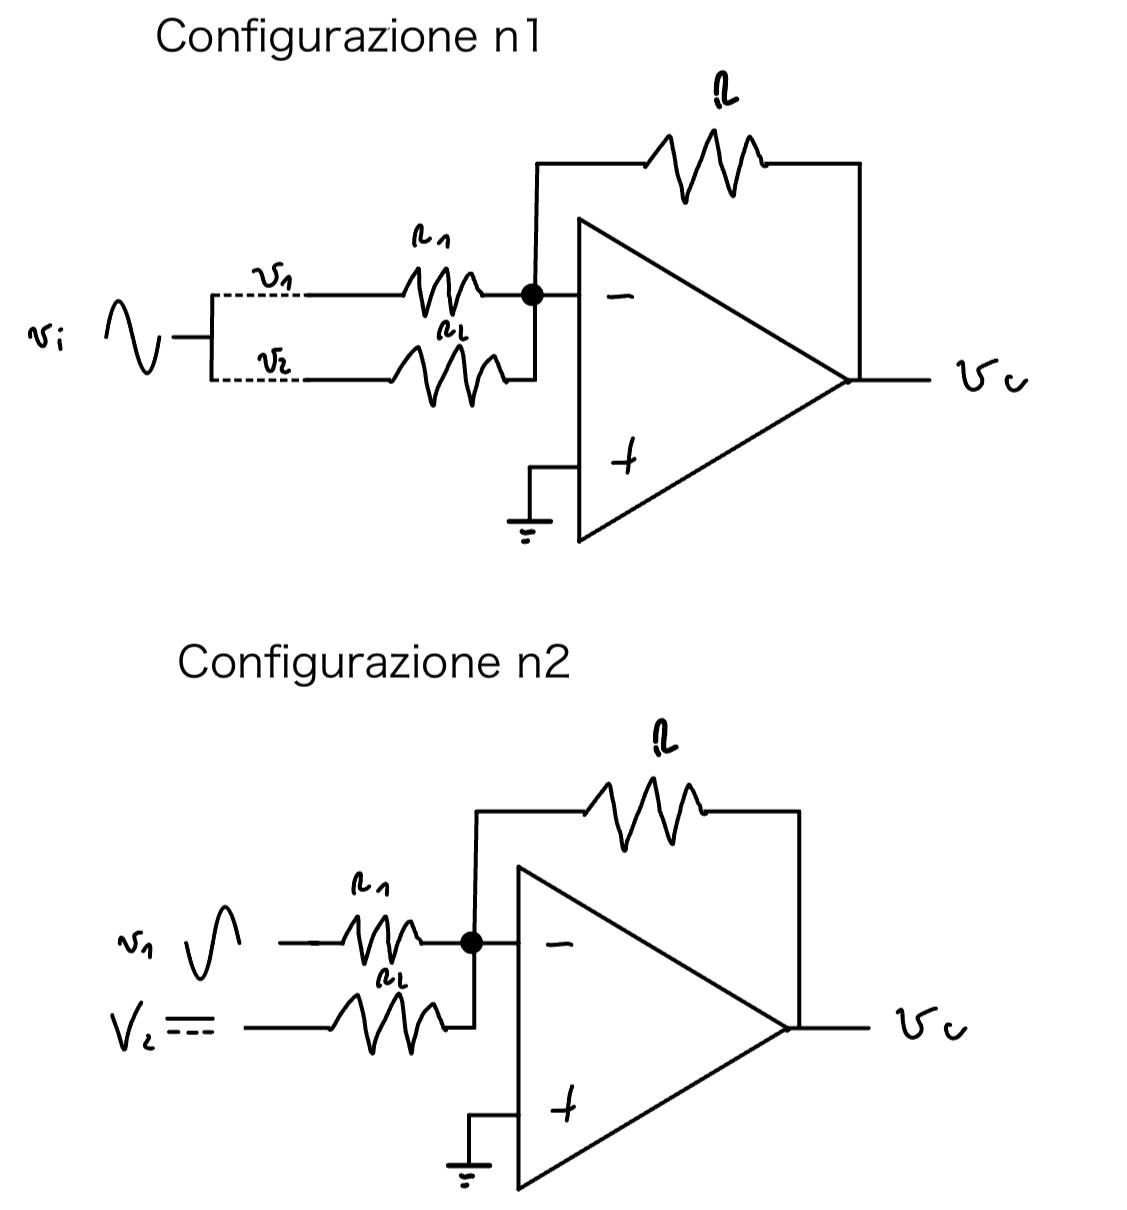
\includegraphics[scale=0.28]{schema.jpg}
\end{flushleft}
\section{Materiale e Strumenti}
\label{Materiale e Strumenti}
\begin{multicols}{2}
    \begin{itemize}
    \item Fili di collegamento
    \item Breadboard
    \item Resistenza da $33k\Omega$
    \item Resistenza da $100k\Omega$
    \item Amplificatore operazionale \textit{U741}
    \end{itemize}
    \vfill\null
    \columnbreak
    \begin{itemize}
    \item Multimetro
    \item Generatore di funzione
    \item Oscilloscopio
    \item Alimentazione DC ($\pm$ 15V)
    \item Alimentatore DC
    \end{itemize}
    \vfill\null
    \end{multicols}
\vspace{15pt}
\section{Contenuti Teorici}
Avendo i valori delle resistenze e delle tensioni in ingresso è possibile calcolare la tensione in uscita.
I valori ottenuti sperimentalmente dovranno essere circa coincidenti al risultato dei calcoli ammettendo
una discrepanza data dai vari errori sistematici.\\
Nella seconda prova vengono sommate una tensione alternata e una tensione continua negativa, tramite l'oscilloscpio
si potrà notare che la somma delle due sarà la tensione continua spostata rispetto all'asse \textit{y} 
della tensione negativa.
\subsection{Descrizione della Prova}
Dopo aver svolto i calcoli teorici vanno misurate le resistenze e verificato che il valore sia com-
parabile a quello riportato tramite codice colore.\\
Dopodichè viene montato il circuito sulla Breadboard seguendo lo schema, prima di collegarlo
all’ alimentazione viene regolata la tensione usando un multimetro come riferimento.\\
Come ultima cosa si collega e si impostano oscilloscopio e generatore di funzione alla tensione $v_i$ con frequenza data.\\
Per il primo circuito le due tensioni di ingresso sono uguali.\\
Si misura la tensione in uscita tramite la funzione \textit{measure} dell'oscilloscopio.\\
Si ripete lo stesso procedimento solo che colleghiamo $v_2$ al generatore di tensione tarato a -2V.\\
Si misura la tensione in uscita e l'offset tramite la funzione \textit{measure} dell'oscilloscopio.\\
\section{Raccolta dei dati}
\subsection{Oscilloscopio}
\begin{figure}[h]
    \centering
    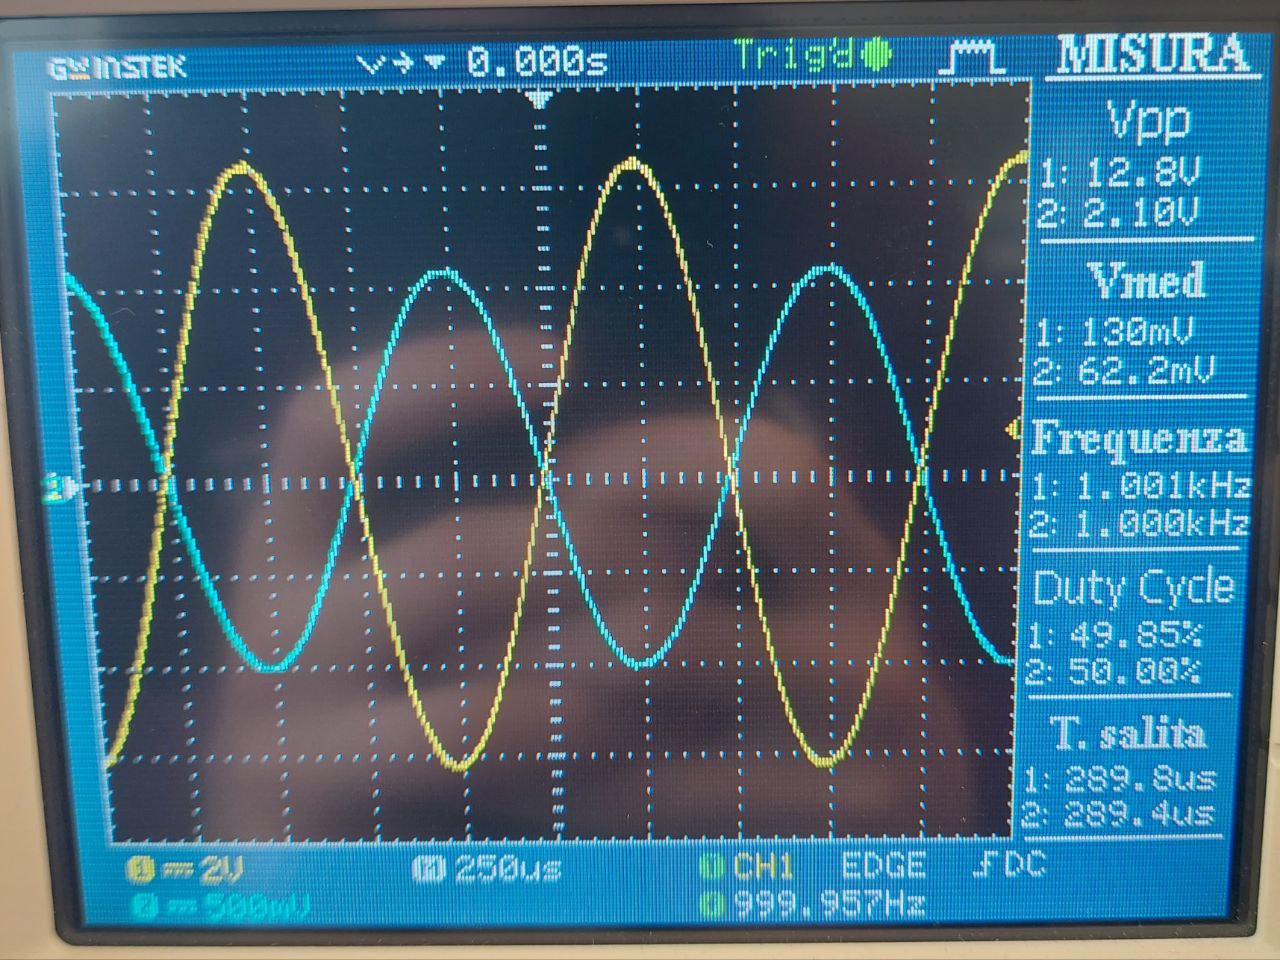
\includegraphics[scale=0.1]{osc1.jpg}
    \caption{Configurazione n1}
\end{figure}
\begin{figure}[h]
    
    \centering
    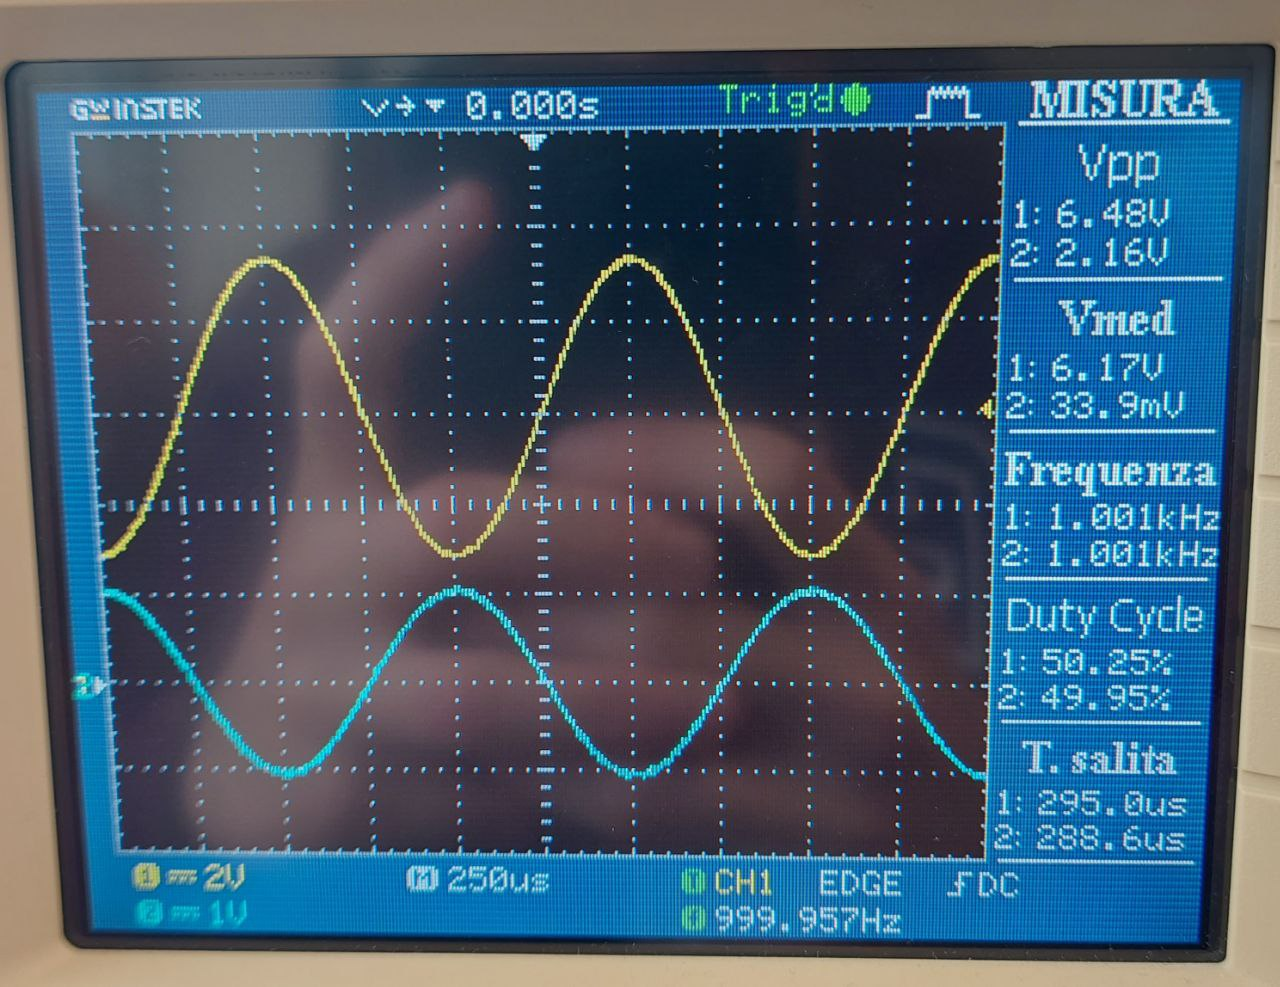
\includegraphics[scale=0.1]{osc2.jpg}
    \caption{Configurazione n2}
\end{figure}
\section{Multisim}
\begin{figure}[h]
    \centering
    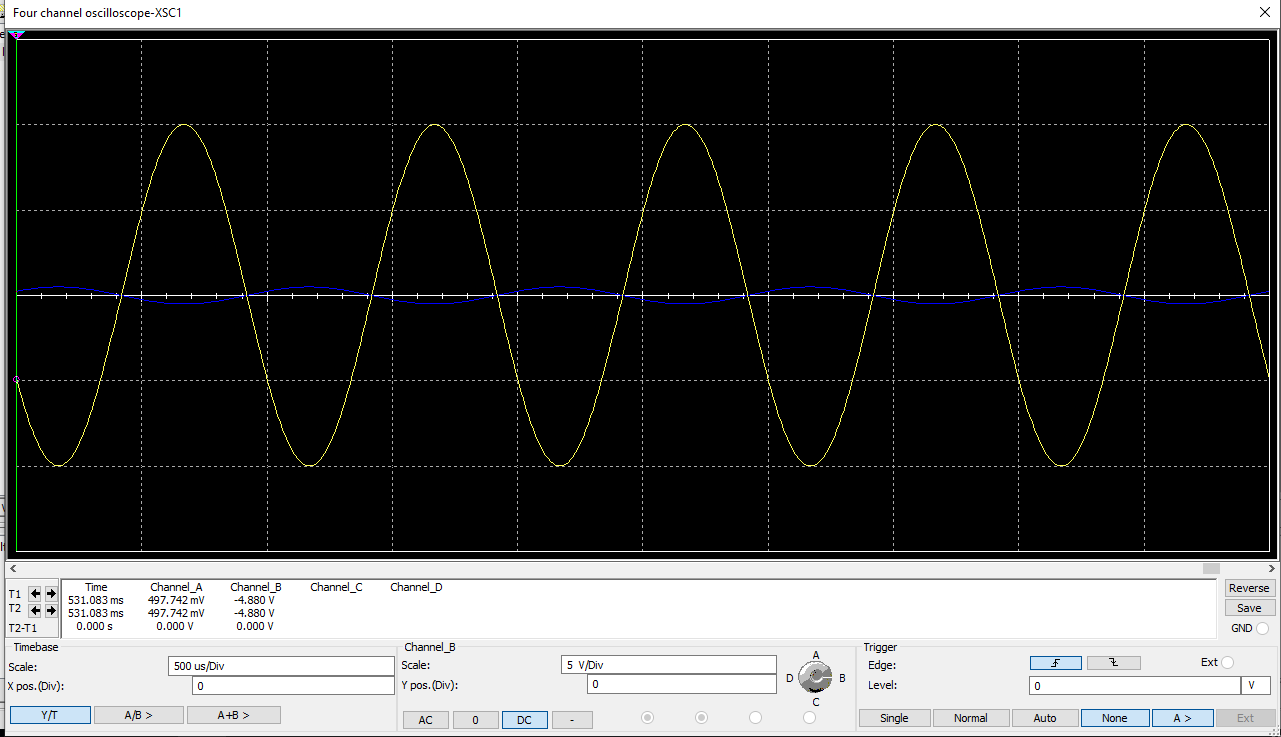
\includegraphics[scale=0.2]{Screenshot (3).png}
    \caption{Sommatore invertente}
\end{figure}
\subsection{Tabella}
Valore misurato resistenze:\\
\begin{center}
        \begin{tabular}{|p{2cm}|p{2cm}|}
            \hline
            \rowcolor{Green} $R_1$ & $R_2$ \\
            \hline
            \rowcolor{LimeGreen} $98k\Omega$ & $32k\Omega$  \\ 
            \hline
        \end{tabular}
        \label{Valore resistenze}
\end{center}
\noindent
Configurazione n°1:\\
\begin{center}
    \begin{tabular}{|p{2cm} |p{2cm}|}
        \hline
        \rowcolor{Green} $V_i$ & $V_o$  \\
        \hline
        \rowcolor{LimeGreen} $1V$ & $-6.4V$  \\ 
        \hline
    \end{tabular}
\end{center}


\noindent Configurazione n°2:\\
\begin{center}
    \begin{tabular}{|p{2cm} |p{2cm}|}
        \hline
        \rowcolor{Green} $V_i$ & $V_o$  \\
        \hline
        \rowcolor{LimeGreen} $1.08V$ & $3.1V$  \\ 
        \hline
    \end{tabular}
\end{center}
\subsection{Commento dei dati raccolti in tabella}
I valori sperimentali delle resistenze rientrano nelle tolleranze.\\
Dall'oscilloscopio si vede che entrambe le tensioni di uscita sono correttamente invertite.\\
La $v_o$ del primo caso corrisponde a quella calcolata.\\
Nel secondo caso si nota che il segnale di uscita è spostato in basso di circa 2V come aspettato.\\
\section{Elaborazione dei dati raccolti}
\subsection{Calcoli}
Configurazione n1:\\
$V_M\sin (\omega t)=1V(2\pi1KHzt)$\\
$v_1=v_2$\\
$v_u=-R(\frac{v_1}{R_1}+\frac{v_2}{R2})=-\frac{R_1}{R_{12}}(v_1+v_2)=-\frac{98k\Omega}{33K\Omega}(1V+1V)=-6V$\\
\\
Configurazione n2:\\
$V_M\sin (\omega t)=1V(2\pi1KHzt)$\\
$V_2=-2V$\\
$v_u=-R(\frac{v_1}{R_1}+\frac{v_2}{R2})=-\frac{R_1}{R_{12}}(v_1+v_2)=-\frac{98k\Omega}{33K\Omega}(1V-2V)=3V$
\section{Analisi critica dei risultati e conclusioni}
Lo scopo è soddisfatto perché i valori di uscita della prima configurazione, della seconda configurazione e dell'offset
della seconda configurazione sono equivalenti a quelle restituite dai calcoli teorici
\end{document}